\documentclass[spanish,a4paper,12pt,oneside]{extreport}

\usepackage[dvips]{graphicx}
\usepackage[dvips]{epsfig}

\usepackage[T1]{fontenc}
\usepackage[utf8]{inputenc}
\usepackage[spanish]{babel}

%\usepackage[latin1]{inputenc}
%\usepackage[spanish]{babel}

\usepackage{alltt}

\usepackage[ruled,vlined,commentsnumbered,linesnumbered,inoutnumbered,titlenotnumbered,noend]{algorithm2e}
\SetKwRepeat{Do}{do}{while}

\usepackage{multirow}
\usepackage{array} 
\usepackage{amsfonts}
\usepackage{amsmath}
\usepackage{bigstrut}
\usepackage{booktabs}
\usepackage{caption}
\usepackage{chngpage}
\usepackage{float}
\usepackage{comment}
%\usepackage{enumitem,lipsum}
\usepackage{graphicx}
\usepackage{lscape}
\usepackage{microtype}
\usepackage{natbib}
\usepackage{pdflscape}
\usepackage{rotating}
\usepackage{subcaption}
\usepackage{ctable}
\usepackage{hyperref}
\usepackage{enumerate}
\usepackage{gensymb}
\usepackage{eurosym}
\usepackage{xcolor}
\usepackage{tabu}
\usepackage[export]{adjustbox}[2011/08/13]
\usepackage{lineno}
\usepackage{epigraph}
%\usepackage[sanitize=none]{glossaries}
\usepackage[toc]{glossaries}

%\\linenumbers
%\setlength\linenumbersep{5pt}
%\renewcommand\linenumberfont{\normalfont\tiny\sffamily\color{gray}}

%\makenoidxglossaries
\makeglossaries

\newglossaryentry{DSL}{
    name={DSL},
    description={
        Un lenguaje específico de dominio (DSL) es un lenguaje que está dirigido a resolver un tipo particular de problema. El uso de DSL es muy común en informática: CSS, expresiones regulares, make, ant, SQL, muchos bits de Rails, expectativas en JMock, el lenguaje graphviz, los archivo de configuración de strut, etc.
    }
}

%\newglossaryentry{GitHub Action}{
%    name={GitHub Action},
%    description={
%        GitHub Actions es una plataforma de integración continua y entrega continua (CI/CD) que permite automatizar la %canalización de tareas como la compilación, pruebas y despliegue, permitiendo crear flujos de trabajo que construyan %nuevos artefactos como publicaciones, releases, imágenes, pdfs, etc.
%    }
%}

\newglossaryentry{JIT}
{
    name=JIT,
    description={just-in-time compiler. También conocido en español como \textbf{compilación en tiempo de ejecución}. Es una forma de ejecutar el código informático que implica la compilación durante la ejecución de un programa (en tiempo de ejecución) en lugar de antes de la ejecución}
}

\newglossaryentry{AOT}
{
    name=AOT,
    description={En informática, la \textbf{compilación anticipada} es el acto de compilar un lenguaje de programación (a menudo) de alto nivel en un lenguaje (a menudo) de bajo nivel antes de la ejecución de un programa, normalmente en tiempo de compilación, para reducir la cantidad de trabajo necesario en tiempo de ejecución.
    De hecho, dado que todas las compilaciones estáticas se realizan técnicamente con antelación, esta expresión en particular se utiliza a menudo para destacar algún tipo de ventajas de rendimiento del acto de dicha precompilación. El acto de compilar Java a bytecode Java es por tanto raramente referido como AOT ya que es normalmente un requisito, no una optimización}
}

\newglossaryentry{API}
{
    name=API,
    description={Una \textbf{interfaz de programación de aplicaciones} es una manera de que dos o más programas informáticos se comuniquen entre sí. Es un tipo de interfaz de software que ofrece un servicio a otras piezas de software}
}

\newglossaryentry{power users}
{
    name=power users,
    description={Un \textbf{usuario avanzado} es un usuario de ordenadores, software y otros dispositivos electrónicos, que utiliza características avanzadas del hardware informático, sistemas operativos, programas o sitios web que no son utilizados por el usuario medio. Un usuario avanzado puede no tener amplios conocimientos técnicos de los sistemas que utiliza, pero se caracteriza más bien por la competencia o el deseo de hacer el uso más intensivo de los programas o sistemas informáticos}
}

\newglossaryentry{cache}
{
    name=caché,
    description={Una \textbf{cache} es un componente de hardware o software que almacena datos para que las futuras solicitudes de esos datos puedan ser atendidas más rápidamente; los datos almacenados en una caché pueden ser el resultado de un cálculo anterior o una copia de datos almacenados en otro lugar}
}

\newglossaryentry{CLI}
{
    name=CLI,
    description={Es un tipo de interfaz de usuario de computadora que permite a los usuarios dar instrucciones a algún programa informático o al sistema operativo por medio de una línea de texto simple}
}

\newglossaryentry{strategy pattern}
{
    name=patrón estrategia,
    description={En programación informática, el patrón de estrategia (también conocido como patrón de política) es un patrón de diseño de software de comportamiento que permite seleccionar un algoritmo en tiempo de ejecución. En lugar de implementar un único algoritmo directamente, el código recibe instrucciones en tiempo de ejecución sobre cuál de una familia de algoritmos utilizar}
}

\newglossaryentry{graceful degradation}{
    name={degradación gradual},
    description={La \textbf{tolerancia a los fallos} es la propiedad que permite a un sistema seguir funcionando correctamente en caso de fallo de uno o varios de sus componentes. A diferencia de un sistema diseñado ingenuamente, en el que incluso un pequeño fallo puede provocar una avería total}
}

\newglossaryentry{namespace}{
    name={espacio de nombre},
    description={En informática, un \textbf{espacio de nombres} es un conjunto de signos (nombres) que se utilizan para identificar y referirse a objetos de diversos tipos. Un espacio de nombres garantiza que todos los objetos de un conjunto determinado tengan nombres únicos para que puedan ser fácilmente identificados}
}

\newglossaryentry{corrutine}{
    name={corrutina},
    description={Las \textbf{corrutinas} son componentes de programas informáticos que generalizan las subrutinas para la multitarea no preferente, permitiendo suspender y reanudar la ejecución}
}

\newglossaryentry{hash}{
    name={hash},
    description={Un \textbf{hash} (que también puede llamarse un condensado o una firma) es un valor calculado a partir de un valor diferente. En la gran mayoría de los casos, este valor está representado en forma de una cadena de caracteres hexadecimales. Los hashs suelen utilizarse para verificar que un archivo no se ha visto corrompido o bien para autentificar a un usuario sin tener que almacenar su contraseña en claro}
}

\newglossaryentry{regex}{
    name={expresión regular},
    plural={expresiones regulares},
    description={Una \textbf{expresión regular} (abreviada como regex o regexp) es una secuencia de caracteres que especifica un patrón de búsqueda en un texto. Los algoritmos de búsqueda de cadenas suelen utilizar estos patrones para las operaciones de "búsqueda" o "búsqueda y sustitución" de cadenas, o para la validación de entradas}
}

\newglossaryentry{deserialization}{
    name={deserializar},
    plural={deserializa},
    description={Extraer una estructura de datos de una serie de bytes}
}

\newglossaryentry{serialization}{
    name={serializar},
    plural={serializa},
    description={Es el proceso de traducir una estructura de datos o el estado de un objeto a un formato que pueda ser almacenado (por ejemplo, en un archivo o en un búfer de datos de la memoria) o transmitido (por ejemplo, a través de una red informática)}
}

\usepackage[top=2cm, bottom=2cm, left=2cm, right=2cm]{geometry}

\newenvironment{sourcecode}
{\begin{list}{}{\setlength{\leftmargin}{1em}}\item\scriptsize\bfseries}
{\end{list}}

\newenvironment{littlesourcecode}
{\begin{list}{}{\setlength{\leftmargin}{1em}}\item\tiny\bfseries}
{\end{list}}

\newenvironment{summary}
{\par\noindent\begin{center}\textbf{Abstract}\end{center}\begin{itshape}\par\noindent}
{\end{itshape}}

\newenvironment{keywords}
{\begin{list}{}{\setlength{\leftmargin}{1em}}\item[\hskip\labelsep \bfseries Keywords:]}
{\end{list}}

\newenvironment{palabrasClave}
{\begin{list}{}{\setlength{\leftmargin}{1em}}\item[\hskip\labelsep \bfseries Palabras clave:]}
{\end{list}}

\usepackage{bera}% optional: just to have a nice mono-spaced font
\usepackage{listings}
\usepackage{xcolor}

\colorlet{punct}{red!60!black}
\definecolor{background}{HTML}{EEEEEE}
\definecolor{delim}{RGB}{20,105,176}
\colorlet{numb}{magenta!60!black}

\lstdefinelanguage{json}{
    basicstyle=\normalfont\ttfamily,
    numbers=left,
    numberstyle=\scriptsize,
    stepnumber=1,
    numbersep=8pt,
    showstringspaces=false,
    breaklines=true,
    frame=lines,
    backgroundcolor=\color{background},
    literate=
     *{0}{{{\color{numb}0}}}{1}
      {1}{{{\color{numb}1}}}{1}
      {2}{{{\color{numb}2}}}{1}
      {3}{{{\color{numb}3}}}{1}
      {4}{{{\color{numb}4}}}{1}
      {5}{{{\color{numb}5}}}{1}
      {6}{{{\color{numb}6}}}{1}
      {7}{{{\color{numb}7}}}{1}
      {8}{{{\color{numb}8}}}{1}
      {9}{{{\color{numb}9}}}{1}
      {:}{{{\color{punct}{:}}}}{1}
      {,}{{{\color{punct}{,}}}}{1}
      {\{}{{{\color{delim}{\{}}}}{1}
      {\}}{{{\color{delim}{\}}}}}{1}
      {[}{{{\color{delim}{[}}}}{1}
      {]}{{{\color{delim}{]}}}}{1},
}

% Configuración de los colores de los enlaces
\hypersetup{
    colorlinks = true,
    linkcolor = blue,
    filecolor = magenta,      
    urlcolor = cyan,
}

\begin{document}

\renewcommand\listtablename{Índice de Tablas}    
\renewcommand\listfigurename{Índice de Figuras}    

%%%%%%%%%%%%%%%%%%%%%%%%%%%%%%%%%%%%%%%%%%%%%%%%%%%%%%%%%%%%%%%%%%%%%%%%%%%%%%%
% First Page
%%%%%%%%%%%%%%%%%%%%%%%%%%%%%%%%%%%%%%%%%%%%%%%%%%%%%%%%%%%%%%%%%%%%%%%%%%%%%%%
\pagestyle{empty}
\thispagestyle{empty}


\newcommand{\HRule}{\rule{\linewidth}{1mm}}
\setlength{\parindent}{0mm}
\setlength{\parskip}{0mm}

\vspace*{\stretch{0.5}}

\begin{center}

\includegraphics[scale=0.8]{images/escuela-ingenieria-tecnologia-original}\\[10mm]
{\Huge Trabajo de Fin de Grado}
\end{center}

\HRule
\begin{flushright}
    {\Huge Extending GitHub CLI with Default Owners} \\[2.5mm]
    {\Large \textit Extendiendo GitHub CLI con Propietarios por Defecto} \\[5mm]
    {\Large Diego Pérez García} \\[5mm]
\end{flushright}
\HRule

\vspace*{\stretch{2}}
\begin{center}
  \Large La Laguna, \today
\end{center}

\setlength{\parindent}{5mm}

%%%%%%%%%%%%%%%%%%%%%%%%%%%%%%%%%%%%%%%%%%%%%%%%%%%%%%%%%%
% Signature page (add the official stamp)
%%%%%%%%%%%%%%%%%%%%%%%%%%%%%%%%%%%%%%%%%%%%%%%%%%%%%%%%%%
\newpage
\thispagestyle{empty}

D. {\bf Casiano Rodríguez León}, con N.I.F. 42.020.072-S  profesor Catedrático de Universidad adscrito al Departamento de Nombre del Departamento de la Universidad de La Laguna, como tutor


\bigskip
\bigskip
{\bf C E R T I F I C A N}

\bigskip
\bigskip
Que la presente memoria titulada:

\bigskip
''{\it Extending GitHub CLI with Default Owners}''

\bigskip
\bigskip
\bigskip

\noindent ha sido realizada bajo su dirección por D. {\bf Diego Pérez García},
con N.I.F. 79081733M.

\bigskip
\bigskip

Y para que así conste, en cumplimiento de la legislación vigente y a los efectos
oportunos firman la presente en La Laguna a \today

%%%%%%%%%%%%%%%%%%%%%%%%%%%%%%%%%%%%%%%%%%%%%%%%%%%%%%%%%%
\newpage
\thispagestyle{empty}

%{ \flushright

\begin{LARGE}
Agradecimientos
\end{LARGE}

\hspace{3mm}

\begin{large}
A mis amigos ya graduados que me han brindado apoyo, consejo y ánimos a pesar de haberme tardado un año más que ellos. \\
A mi mejor amiga por brindarme el mayor de los apoyos cuando tuve que repetir asignaturas. \\
A su vez a mis compañeros por esta gran experiencia y esos recuerdos que me llevo de mi vida universitaria. \\
A los profesores Francisco de Sande González, Marcos Colebrook-Santamaria, Iván Castilla Rodríguez y Albano José González Fernández por su gran labor como profesores demostrando cada año que tratan de llegar a los alumnos para transmitir sus conocimientos de la mejor manera. \\
A mi familia que me ha permitido centrarme en los estudios que me han llevado a ser el programador que soy hoy. \\
Y por último a mi tutor Casiano Rodríguez León por ofrecer esta oportunidad de proyecto y aprendizaje, a la vez de ser un profesor con paciencia y que me ha permitido sacar el mejor resultado. \\
\end{large}

%}
%%%%%%%%%%%%%%%%%%%%%%%%%%%%%%%%%%%%%%%%%%%%%%%%%%%%%%%%
\newpage
\thispagestyle{empty}

\bigskip
\begin{LARGE}
Licencia
\end{LARGE}

\begin{center}

\includegraphics[scale=1.8]{images/by_88x31}\\[5mm]
\end{center}

\begin{large}
© Esta obra está bajo una licencia de Creative Commons Reconocimiento 4.0 Internacional.
\end{large}

%%%%%%%%%%%%%%%%%%%%%%%%%%%%%%%%%%%%%%%%%%%%%%%%%%%%%%%%
\newpage 
\thispagestyle{empty}

\begin{abstract} % TODO: Revisar ortografía
Está muy arraigado en la informática el uso de GitHub como plataforma de enseñanza.
Dando paso a herramientas claves como GitHub Classroom con soporte para asignar tareas de manera fácil
y sencilla. Por otra parte la plataforma ofrece una herramienta llamada GitHub CLI que permite interactuar 
con esta por medio de  de la línea de comandos.

Este trabajo presenta un comando nuevo para la GitHub CLI 
denominado \verb|gh owner| que tiene como objetivo romper con un problema 
de experiencia de usuario que es tener que recordar los largos y varios OWNERS 
que pueda tener un usuario en su cuenta. Esto resuelve entonces una cantidad de comandos 
que requieren de pasar como argumento OWNER/REPO, por lo que declarar un OWNER por defecto y simplemente pasar REPO resulta en combinar este OWNER con el REPO para generar un argumento completo y más fácil de rellenar.
\begin{palabrasClave}
github-cli, github-education, graphql, rest, git, go
\end{palabrasClave}

\end{abstract}
%%%%%%%%%%%%%%%%%%%%%%%%%%%%%%%%%%%%%%%%%%%%%%%%%%%%%%%%%
\newpage 
\vspace*{200px}
\thispagestyle{empty}

\begin{summary} % TODO: Traducir
\begin {keywords}
github-cli, github-owners, graphql, rest, git, terminal, go
\end {keywords}

\end{summary}
%%%%%%%%%%%%%%%%%%%%%%%%%%%%%%%%%%%%%%%%%%%%%%%%%%%%%%%%%
\newpage{\pagestyle{empty}}
\thispagestyle{empty}

%%%%%%%%%%%%%%%%%%%%%%%%%%%%%%%%%%%%%%%%%%%%%%%%%%%%%%%%%
\pagestyle{myheadings} %my head defined by markboth or markright
% No funciona bien \markboth sin "twoside" en \documentclass, pero al
% ponerlo se dan un montón de errores de underfull \vbox, con lo que no se
% ha puesto.


%%Aqui debería poner el nombre del proyecto pero, como es muy grande no cabe y se ve feo en el PDF
\markboth{xxxxx}{}

%%%%%%%%%%%%%%%%%%%%%%%%%%%%%%%%%%%%%%%%%%%%%%%%%%%%%%%%%
%Numeracion en romanos
\renewcommand{\thepage}{\roman{page}}
\setcounter{page}{1}
\pagestyle{plain} 

%%%%%%%%%%%%%%%%%%%%%%%%%%%%%%%%%%%%%%%%%%%%%%%%%%%%%%%%%

{\hypersetup{linkcolor=black}
\tableofcontents

%%%%%%%%%%%%%%%%%%%%%%%%%%%%%%%%%%%%%%%%%%%%%%%%%%%%%%%%%
\newpage{\pagestyle{empty}}

\listoffigures

%%%%%%%%%%%%%%%%%%%%%%%%%%%%%%%%%%%%%%%%%%%%%%%%%%%%%%%%%
\newpage{\pagestyle{empty}}

\listoftables
}

%%%%%%%%%%%%%%%%%%%%%%%%%%%%%%%%%%%%%%%%%%%%%%%%%%%%%%%%%%%%%%%%%%%%%%%%%%%%%%%
\newpage{\pagestyle{empty}}

%%%%%%%%%%%%%%%%%%%%%%%%%%%%%%%%%%%%%%%%%%%%%%%%%%%%%%%%%%%%%%%%%%%%%%%%%%%%%%%
\newpage
\thispagestyle{empty}

%Numeracion a partir del capitulo I
\renewcommand{\thepage}{\arabic{page}}
\setcounter{page}{1}
\pagestyle{plain}

\chapter{\LARGE Introducción, Antecedentes y Estado del Arte}
\label{chapter:intro}

%\section{Motivación}
\section{Introducción}
%Repetir aquí el proyecto de TFG
Durante muchos años, profesores de programación de todo el mundo han utilizado y siguen utilizando GitHub como plataforma para la enseñanza de asignaturas relacionadas con la programación, el trabajo en equipo y el desarrollo de proyectos. La propia empresa GitHub ha apoyado estas iniciativas dentro de un grupo de acciones que se inscriben bajo el término  GitHub Education. Ello incluye descuentos en plataformas y herramientas para profesores y alumnos, foros específicos de discusión, congresos, becas, y herramientas específicas. Entre estas últimas cabe señalar  GitHub Classroom, la cual da soporte al proceso de asignación de tareas.

Hace solo dos años GitHub introdujo una herramienta denominada GitHub CLI (a veces referenciada como gh-cli o gh). Es una herramienta de código abierto para utilizar los servicios que provee GitHub, pero desde la línea de comandos.  Es posible ver, crear, clonar, y bifurcar repositorios; crear, cerrar, editar y ver incidencias, etc. Sin embargo el conjunto de funcionalidades  ofrecido es aún bastante menor que el disponible en la interfaz web.

En agosto del año 2021 los desarrolladores de GitHub Cli añadieron un mecanismo denominado gh-cli extensions (denominado gh-extensions) que facilita que terceros puedan añadir nuevas funcionalidades a gh-cli mediante un repositorio GitHub.


\section{Antecedentes y estado actual del tema}
Uno de los primeros intentos en integrar GitHub al mundo educativo fue \href{https://github.com/education/teachers_pet}{“teachers\_pet”}, una herramienta de la línea de comandos que ayudaba al profesorado a impartir sus clases intentando emular una plataforma de aprendizaje. Cada clase era una organización de GitHub y los alumnos estaban repartidos en equipos en los que estaban solo ellos mismos, de esta manera los profesores podían gestionar todos los repositorios de la organización, dar plantillas con las que los alumnos podían empezar a trabajar, comprobar el progreso, etc.
 Más tarde, GitHub respondería a la demanda con Github Classroom  un servicio web de uso más intuitivo que dejaría obsoleto a \verb|teacher's pet|, y que a día de hoy es la más utilizada.

En lo referente al GitHub CLI ya existía con anterioridad, una herramienta antecesora similar que proveía funcionalidades similares, fue  llamada \verb|hub|, actualmente mantenida por Mislav Marohnić (empleado de GitHub, Inc.). Hub fue creado originalmente por Chris Wanstrath, que junto con Tom Preston, Scott Chacon y P.J. Hyett fundaron GitHub en 2008. al igual que GitHub CLI esta herramienta nos permite interactuar con Github desde la terminal, pero esta se podría considerar un producto personal y más centrado en los denominados \gls{power users}. El 20 de febrero de 2020 Github anuncia Github CLI, el sucesor de hub mantenido y en desarrollo por un equipo oficial de la compañía y más amigable de usar. El 20 de agosto de 2021 sale la versión 2.0 con el comando \verb|extension|\cite{gh-extension}, con la cual los usuarios podrán crear sus propias extensiones que nos permiten generar por nosotros mismos y con relativa facilidad servicios y herramientas que se integren bien con las implementaciones actuales usando  las \gls{API}s de GitHub \verb|REST API|\cite{github-rest-api} y GitHub GraphQL\cite{github-graphql}.

Actualmente, existen cientos de extensiones dirigidas al desarrollador, pero son pocas las que están dedicadas a facilitar la gestión de las organizaciones, en especial aquellas dedicadas a la enseñanza. Este proyecto tiene como objetivo crear una extensión modular de GitHub CLI que complementa a GitHub classroom y que provee funcionalidades como:

\begin{itemize}
    \item Creación y asignación de tareas
    \item Seguimiento del progreso de los miembros de la organización
    \item Soporte a la gestión de incidencias
    \item Facilitar la retroalimentación a los trabajos realizados por los alumnos
    \item Interoperabilidad entre subcomandos para permitir comportamientos más complejos
    \item Interfaz rápida y amigable
\end{itemize}

%%%%%%%%%%%%%%%%%%%%%%%%%%%%%%%%%%%%%%%%%%%%%%%%%%%%%%%%%%%%%%%%%%%%%%%%%%%%%%%
\newpage{\pagestyle{empty}}
\thispagestyle{empty}

\chapter{\LARGE Tecnologías}
\label{chapter:dos}

En el desarrollo de proyectos informáticos, existe una amplia gama de tecnologías disponibles que abarcan desde herramientas de control de versiones y plataformas de colaboración hasta lenguajes de programación y sistemas de preparación de documentos. La selección de las tecnologías adecuadas es crucial para asegurar la eficiencia, la escalabilidad y el éxito del proyecto. A continuación, se describen las principales tecnologías utilizadas en el desarrollo del comando gh owner para la GitHub CLI, proporcionando una visión general de sus características y su relevancia para el proyecto.

\section{GitHub}
GitHub es una plataforma de desarrollo colaborativo que utiliza Git para el control de versiones. Fundada en 2008, se ha convertido en una de las herramientas más populares para la gestión de proyectos de software, ofreciendo funcionalidades como la integración continua, el seguimiento de problemas, y la revisión de código. GitHub permite a los desarrolladores trabajar en conjunto de manera eficiente, manteniendo un historial completo de los cambios en el código.

\subsection{GitHub CLI} 
GitHub CLI, lanzada en febrero de 2020, es una herramienta de línea de comandos que permite a los usuarios interactuar con GitHub directamente desde su terminal. Esta herramienta facilita muchas operaciones comunes en GitHub, como clonar repositorios, gestionar issues y pull requests, y ver el estado de los repositorios. Al ofrecer una interfaz de línea de comandos, GitHub CLI permite a los desarrolladores integrar las funcionalidades de GitHub en sus scripts y flujos de trabajo automatizados, mejorando la eficiencia y la productividad.

Las capacidades de GitHub CLI pueden ser extendidas mediante la creación de comandos personalizados y plugins. Esto permite a los desarrolladores adaptar la herramienta a sus necesidades específicas, incorporando nuevas funcionalidades que mejoran la experiencia del usuario y resuelven problemas específicos, como el comando `gh owner` que simplifica la gestión de nombres de propietarios predeterminados.

\subsection{Las APIs de GitHub: REST y  GraphQL}
La API de GitHub proporciona un acceso programático a muchas de las funciones disponibles en la interfaz web de GitHub. A través de la \verb|API REST| \cite{rest-api} y \verb|GraphQL| \cite{graphql-api}, los desarrolladores pueden realizar operaciones como la creación y gestión de repositorios, la administración de issues y pull requests, y la consulta de datos sobre usuarios y organizaciones.

La API de GitHub es una pieza fundamental en la extensión de GitHub CLI, permitiendo que los comandos personalizados interactúen con GitHub de manera efectiva. Al utilizar la API, los desarrolladores pueden automatizar tareas y construir herramientas que aprovechen la amplia funcionalidad de GitHub, mejorando así la eficiencia y la capacidad de gestión de sus proyectos.

\section{Lenguaje GO}
GO, también conocido como \verb|Golang| \cite{go-lang}, es un lenguaje de programación desarrollado por Google en 2007. Es conocido por su simplicidad, eficiencia y capacidad para manejar la concurrencia de manera efectiva. GO ha sido adoptado ampliamente en el desarrollo de software de sistemas y aplicaciones de red debido a su rendimiento y facilidad de uso.

El comando `gh owner` ha sido desarrollado utilizando GO, aprovechando sus características de concurrencia y su eficiencia en la ejecución. La decisión de utilizar GO se tomó debido a que la GitHub CLI está escrita en este lenguaje, lo que asegura una integración nativa y fluida con la herramienta existente.

\section{Overleaf y  \LaTeX{}}
Overleaf es una plataforma de escritura y colaboración en línea que utiliza  \LaTeX{}, un sistema de preparación de documentos de alta calidad.  \LaTeX{} es ampliamente utilizado en la elaboración de documentos académicos, técnicos y científicos debido a su capacidad para manejar la composición de textos complejos y la inclusión de fórmulas matemáticas.

En este trabajo, \verb|Overleaf y  LaTeX| \cite{latex-overleaf} se utilizan para la redacción y formateo de la documentación técnica. La combinación de estas herramientas permite una colaboración eficiente y una presentación profesional de los resultados del proyecto.  \LaTeX{} proporciona un control preciso sobre el diseño y la tipografía, asegurando que el documento final cumpla con los estándares académicos y profesionales requeridos.

Esta sección proporciona una descripción detallada de las tecnologías empleadas, resaltando sus características clave y su relevancia para el desarrollo del comando `gh owner` y la documentación del proyecto.

%%%%%%%%%%%%%%%%%%%%%%%%%%%%%%%%%%%%%%%%%%%%%%%%%%%%%%%%%%%%%%%%%%%%%%%%%%%%%%%
\newpage{\pagestyle{empty}}
\thispagestyle{empty}

\chapter{\LARGE Modo de uso}
\label{chapter:modo-de-uso}

En este capítulo se explica como se utiliza el ecosistema, con intención de que se pueda entender el propósito de cada extensión. En los capítulos siguientes se entrará en más detalle con respecto a la toma de decisiones en el diseño y como se ha logrado implementar todo el ecosistema 

\section{El Núcleo de {\tt gh edu}: Core}

El diseño de la extensión \verb|gh-edu| sigue el \gls{strategy pattern} y consta de un código núcleo (\verb|core|) que coordina las estrategias y extensiones. Algunas de las estrategias más básicas forman parte del código núcleo que se provee con la \verb|gh-extension| \verb|gh-edu|.

Todos los comandos de \verb|gh-edu|  se pueden ejecutar desde la línea de comandos y cuando es apropiado cuentan con un modo interactivo. La figura \ref{fig:ghEduHelp} muestra los subcomandos disponibles en el núcleo.

\begin{figure}[h]
    \centering
    \makebox[\textwidth][c]{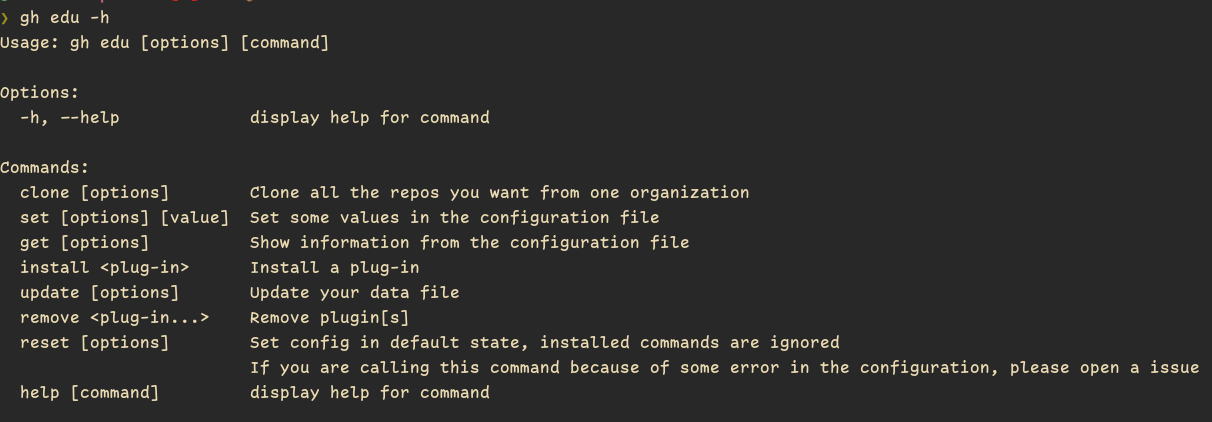
\includegraphics[width=\textwidth]{images/gh-edu-help.png}}
    \caption{Ayuda general de gh edu}
    \label{fig:ghEduHelp}
\end{figure}

Para este apartado es relevante saber que \verb|gh-edu| trabaja en torno a un archivo de datos o registro llamado \verb|data.json|.

Este archivo de datos guarda información
\begin{itemize}
    \item de las extensiones instaladas 
    \item de la versión y configuración de las extensiones instaladas,
    \item de información proveida por las extensiones a solicitud del usuario
    \item del usuario y de la configuración del usuario 
    \item del estado actual del sistema \verb|gh-edu| (por ejemplo, cuál es la organización GitHub por defecto)
    \item de datos obtenidos desde la API de GitHub y que han sido cacheados
\end{itemize}
 este fichero se guarda de forma persistente en \verb|$HOME/.config/gh-edu/data.json|. Este directorio esta siempre bajo control de versiones y puede estar enlazado a un remoto llamado \verb|https://github.com/github-user:/gh-edu-profile|.

Dicho fichero es único y privado para cada usuario y se obtiene de una de estas dos formas:
\begin{itemize}
    \item Se crea uno nuevo a partir de una plantilla base, la cual tiene los elementos mínimos para dar el fichero por válido, o 
    \item Se descarga automáticamente si el usuario tiene uno propio dentro de un repositorio en GitHub en su cuenta con el nombre \verb|<github-user>/gh-edu-profile|. 
\end{itemize}

Se entrará más en detalle sobre \verb|data.json| en el capítulo \textbf{Diseño} \ref{diseño:data}.

\subsection{Subcomando set}
Comando importante, utilizado para establecer la configuración en el fichero de datos
\begin{figure}[h]
    \centering
    \makebox[\textwidth][c]{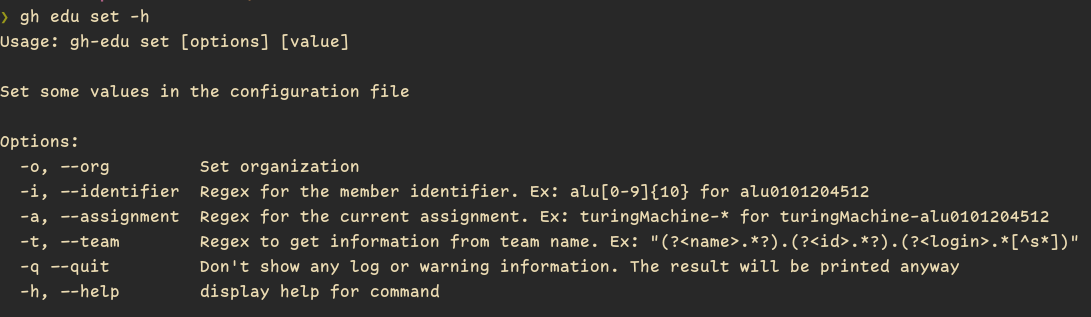
\includegraphics[width=\textwidth]{images/set-help.png}}
    \caption{Ayuda de gh edu set}
    \label{fig:ghEduSetHelp}
\end{figure}

\begin{itemize}
    \item \textbf{-o, -{}-org.} Específica la organización con la que estamos trabajando actualmente. En la mayoría de universidades, las organizaciones de GitHub suelen estar asociados a las asignaturas.
    Ejemplo de uso: \verb|gh edu set -o gh-cli-for-education|, si pertenecemos a la organización se registrará como organización actual y se guardará como cache a los miembros pertenecientes de la organización.
    Si no se le pasa un valor, se activará \verb|fzf| para poder elegir entre las organizaciones a las que el usuario pertenezca.
    \item \textbf{-q, -{}-quiet.} No se muestra ninguna información por pantalla, más allá del resultado y los errores.
    \item \textbf{-i, -{}-identifier.} Expresión regular para identificar los identificadores de los alumnos, en el caso de la ULL utilizamos \verb|alu| seguido de 10 números del 0 al 9. que se corresponde con la expresión regular \verb|alu[0-9]\{10\}|
    \item \textbf{-t, -{}-team.} Expresión regular para poder extraer información del nombre de los equipos. Está pensada para que se utilice con agrupamientos con nombre (``named captured group``). Por ejemplo, la expresión regular:\\ \verb|(?<name>.*?).(?<id>.*?).(?<login>.*[^s*])|\\
    Aplicada sobre el siguiente nombre de equipo:\\
    \verb|cristo-garcia-gonzález.alu0101204512.ggcristo|\\
    Es capaz de generar automáticamente la siguiente información:
    \begin{itemize}
        \item \textbf{name:} cristo-garcia-gonzález
        \item \textbf{id:} alu0101204512
        \item \textbf{login:} ggcristo
    \end{itemize}
    \item \textbf{-a, -{}-assignment}. Expresión regular para marcar los repositorios sobre los que se quiere trabajar. Normalmente, se le asigna un repositorio a cada alumno por asignación/tarea. Por ejemplo: \verb|turingMachine-.*| en el caso de que los repositorios empiecen por \verb|turingMachine| como podría ser \verb|turingMachine-alu0101204512|.
\end{itemize}
El uso que se les dé a estos campos depende deliberadamente de cada desarrollador y profesor.

\subsection{El subcomando core {\tt get}}
\begin{figure}
    \centering
    \makebox[\textwidth][c]{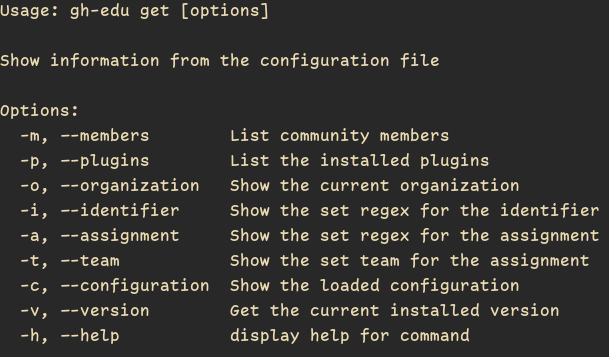
\includegraphics[width=\textwidth]{images/get-help.png}}
    \caption{Ayuda de gh edu get}
    \label{fig:ghEduGetHelp}
\end{figure}
El comando \verb|get| muestra la información que se tiene actualmente
\begin{itemize}
    \item \textbf{-m, -{}-members.} Muestra los miembros de la organización establecida. Lee de la caché, si es posible.
    \item \textbf{-p, -{}-plugins.} Lista las extensiones y comandos disponibles tanto los que vienen con el core (builtin) como los instalados por el usuario.
    \item \textbf{-o, -{}-org.} Muestra la organización marcada.
    \item \textbf{-i, -{}-identifier}. Muestra la expresión regular establecida para detectar los identificadore de los alumnos.
    \item \textbf{-a, -{}-assignment.} Muestra la expresión regular establecida para filtrar los repositorios deseados.
    \item \textbf{-t, -{}-team.} Muestra la expresión regular establecida para recolectar información de los nombres de los equipos.
    \item \textbf{-v, -{}-version.} Muestra la versión instalada.
    \item \textbf{-c, -{}-configuration.} Muestra por pantalla la toda la configuración y datos cargados.
\end{itemize}

\subsection{El subcomando core {\tt clone}}
El comando \verb|clone| solo tiene dos opciones \verb|--org| por si queremos clonar de una organización en concreto sin tener que cambiar la organización establecida y \verb|--quiet| para solo mostrar los mensajes de errores (y \verb|--help|).
Este comando fue planeado para clonar varios repositorios en paralelo usando la librería \href{https://www.npmjs.com/package/concurrently}{concurrently}

\begin{figure}[H]
    \centering
    \makebox[\textwidth][c]{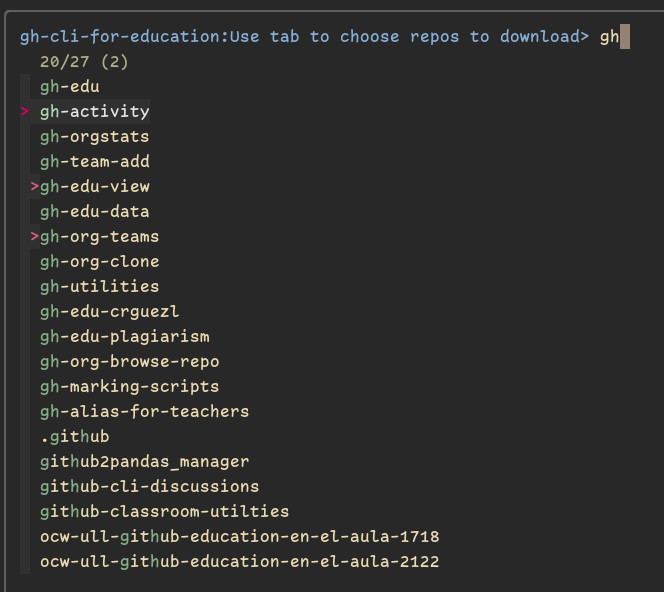
\includegraphics[width=\textwidth]{images/clone.png}}
    \caption{clone usando fzf}
    \label{fig:clone}
\end{figure}

En la figura \ref{fig:clone} se ve la interfaz de \verb|clone| con \verb|fzf|, arriba a la izquierda aparece el nombre de la organización y podemos seleccionar múltiples repositorios presionando \emph{TAB} y filtrarlos de forma difusa (nótese como \verb|.github|, el cual no es una coincidencia exacta, aparece en la lista), para aceptar se pulsa \emph{ENTER}.

\subsection{El subcomando {\tt install}}
Como su nombre indica \verb|install| instala extensiones añadiendo más comandos al sistema. No acepta otro argumento más que el nombre de la extensión que queremos instalar y solamente tiene el \verb|flag| \verb|--quiet|, con la misma funcionalidad que el resto de extensiones.

El código de las extensiones tiene que estar alojado en GitHub y solo funciona con la rama por defecto.

El comando se ejecuta de la siguiente forma:\\
\verb|gh edu install <organización/nombre_extension>|

Ejemplo:

\begin{verbatim}
        gh edu install crguezl/gh-edu-browse
        Installing crguezl/gh-edu-browse ...
        Plugin installed in system
        Setting up configuration...
        crguezl/gh-edu-browse installed as browse
\end{verbatim}
Pero si la extensión es \emph{first-party}, es decir, pertenece a la organización \verb|gh-cli-for-education|, no es necesario especificar la organización. Por ende:\\
\verb|gh edu install gh-cli-for-education/view|, es equivalente a \verb|gh edu install view|

\subsection{El subcomando {\tt remove}}
Elimina las extensiones instaladas por el comando \verb|install|. No puede eliminar los comandos \emph{bultin}.\\
El comando se ejecuta de la siguiente forma:\\
\verb|gh edu remove <nombre_extension1> <nombre_extension2> ... <nombre_extensionN>|

\subsection{El subcomando {\tt update}}

\begin{figure}[htb]
    \centering
    \makebox[\textwidth][c]{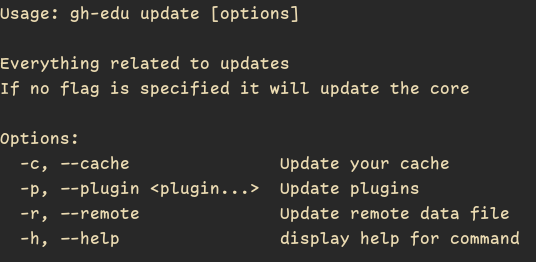
\includegraphics[width=\textwidth]{images/updateHelp.png}}
    \caption{Ayuda de get update}
    \label{fig:updateHelp}
\end{figure}

El subcomando \verb|update| se encarga de todo lo relacionado con las actualizaciones.
\begin{itemize}
    \item \textbf{-c, -{}-cache.} Actualiza todos los valores posibles de la caché. No es un comando esencial, especialmente cuando algunos comandos ya actualizan ciertas partes de la caché, pero es recomendable correrlo desde que se obtenga el fichero de datos data.json.
    \item \textbf{-p, -{}-plugin.} Actualiza una o varías extensiones. Si no tiene un argumento, actualiza todas las extensiones instaladas.
    \item \textbf{-r -{}-remote.} Actualiza el repositorio gh-edu-profile con los datos locales. En caso de no existir se le pregunta al usuario si quiere crear dicho repositorio.
    \item \textbf{Sin argumentos ni \emph{flags}.} Si el usuario ejecuta el comando sin argumentos, el propio \verb|core| se actualizará. Es equivalente a \verb|gh extension upgrade gh-edu|. Fue creado para mantener la simetría con el resto de comandos.
\end{itemize}

\subsection{El subcomando {\tt reset}}
Restaura la configuración a su estado original dejando intacto la información sobre los comandos instalados, si también se desea borrar dicha información se puede usar el flag \verb|--force|, aunque no es recomendable, ya que generaría una incongruencia con las extensiones que están realmente instaladas en el sistema y la propia información del sistema.

Este comando existe por meros motivos de depuración y en caso de que un error en la implementación del sistema lleve al usuario a un estado anormal. No se debe de usar con regularidad.

\section{La Extensión {\tt view}}
Es una pequeña extensión para mostrar información relevante sobre la organización, por lo que es necesario tener una organización establecida.

Dentro del contexto del TFG se ha desarrollado un único comando \verb|members| que muestra información sobre los miembros de la organización. Se espera ampliarlo para que también muestre otro tipo de información que pueda ser relevante al profesorado y alumnado (vease \ref{conclusion}).

Esta extensión también aprovecha la expresión regular del identificador guardado en data.json para intentar conseguir los identificadores de los alumnos leyendo varios campos en su cuenta de GitHub

Se puede ejecutar directamente como: \verb|gh edu view members| o añadir el flag \verb|--id| para usar un identificador que tendrá prioridad sobre el establecido en \verb|data|.
\begin{figure}[H]
    \centering
    \makebox[\textwidth][c]{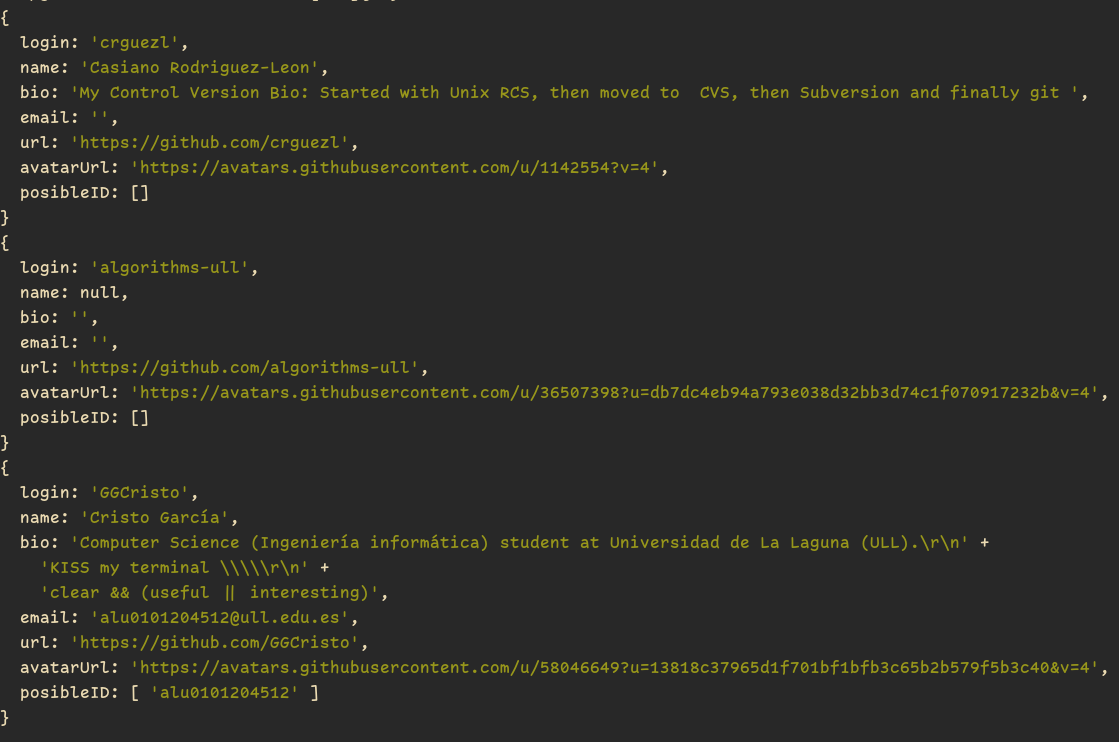
\includegraphics[width=\textwidth]{images/view.png}}
    \caption{Ejemplo de uso de gh view con --id ``alu[0-9]\{10\}``}
    \label{fig:view}
\end{figure}

\section{La Extensión {\tt data}}

Ha sido creado para manejar y guardar información variada de los alumnos.

Para instalarla:
\begin{verbatim}
    gh edu install data
\end{verbatim}

Tiene tres comandos principales: \verb|log|, \verb|teams| y \verb|team-add|:


\begin{verbatim}
    $ gh edu data -h
    Usage: gh-edu-data [options] [command]
    
    Options:
      -h, --help                 display help for command
    
    Commands:
      log [options] <inputFile>  Get relevant information about you students
      teams [options]            Get relevant information about you students using
                                 teams
      team-add [options]         Create teams with certain patterns to get
                                 information later on. Empty spaces will become '-'
      help [command]             display help for command
\end{verbatim}

\subsection{El subcomando {\tt log}}
El objetivo de \verb|log| es principalmente relacionar la cuenta institucional de un alumno con su cuenta de GitHub y conseguir información extra que le pueda ser de utilidad al profesor.

\begin{verbatim}
    gh edu data log -h
    Usage: gh-edu-data log [options] <inputFile>
    
    Get relevant information about you students
    
    Options:
      -o, --output <outputFile>  File to write the resulting data. If not specified
                                 it will write the result to the standard output
      -c, --cache                Cache the information in the configuration file
      -q, --quiet                Don't show any output, except errors
      -h, --help                 display help for command
\end{verbatim}
Se necesita de un fichero inicial con información que el profesor tenga de los alumnos. Dicho fichero de entrada tiene que ser de tipo \verb|JSON|, con un \emph{array} donde cada elemento guarde información de los alumnos. Esta información tiene que contener mínimamente el nombre del alumno, aunque lo apropiado es que contenga el nombre y un identificador. Puede tener más datos (figura \ref{fig:inputJSON}).

Una vez ejecutado el comando, el profesor decide que campos quiere tener de cada alumno (figura \ref{fig:data-desiredData}). Y cuáles de los campos entrantes corresponden al nombre, y en caso de haberlo el identificador (figura \ref{fig:linkFields}). Después, uno a uno y aprovechando la eficaz interfaz de \verb|fzf| y la previsualización de los datos remotos del alumno, se filtra el alumno en cuestión (figura \ref{fig:interface-log}).

Como resultado se obtiene un nuevo fichero JSON que contiene la información dada inicialmente por el profesor, combinada con los datos proporcionados por GitHub (figura \ref{fig:result-log}).

\begin{figure}[H]
    \centering
    \makebox[\textwidth][c]{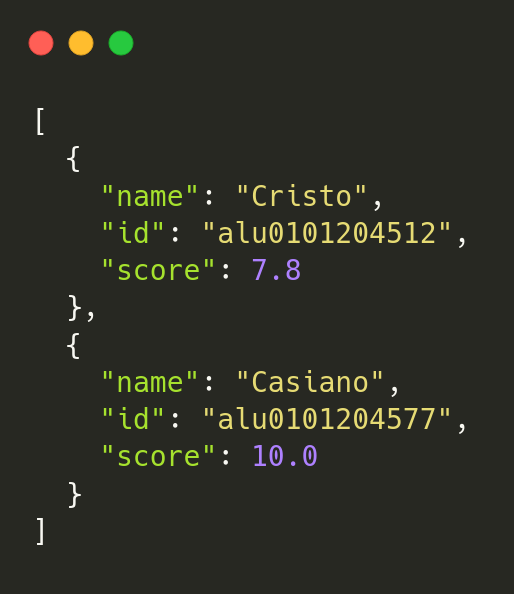
\includegraphics[width=0.5\textwidth]{images/inputJSON.png}}
    \caption{gh edu data log. Ejemplo de archivo de entrada}
    \label{fig:inputJSON}
\end{figure}

\begin{figure}[H]
    \centering
    \makebox[\textwidth][c]{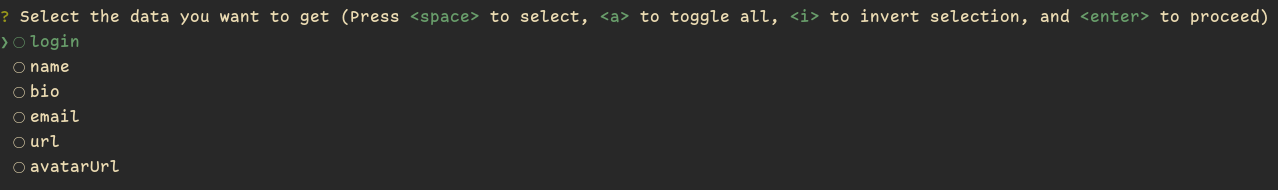
\includegraphics[width=\textwidth]{images/data-select-desiredField.png}}
    \caption{gh edu data log. Seleccionando los datos deseados}
    \label{fig:data-desiredData}
\end{figure}

\begin{figure}[H]
    \centering
    \makebox[\textwidth][c]{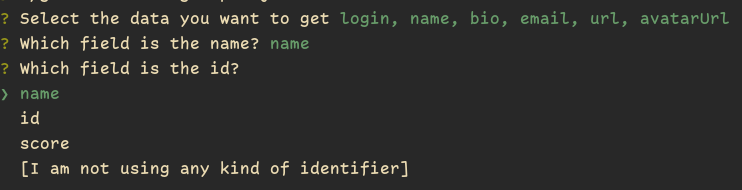
\includegraphics[width=\textwidth]{images/selectFields.png}}
    \caption{gh edu data log. Enlazando los campos del fichero de entrada con el nombre y el ID}
    \label{fig:linkFields}
\end{figure}

\begin{figure}[H]
    \centering
    \makebox[\textwidth][c]{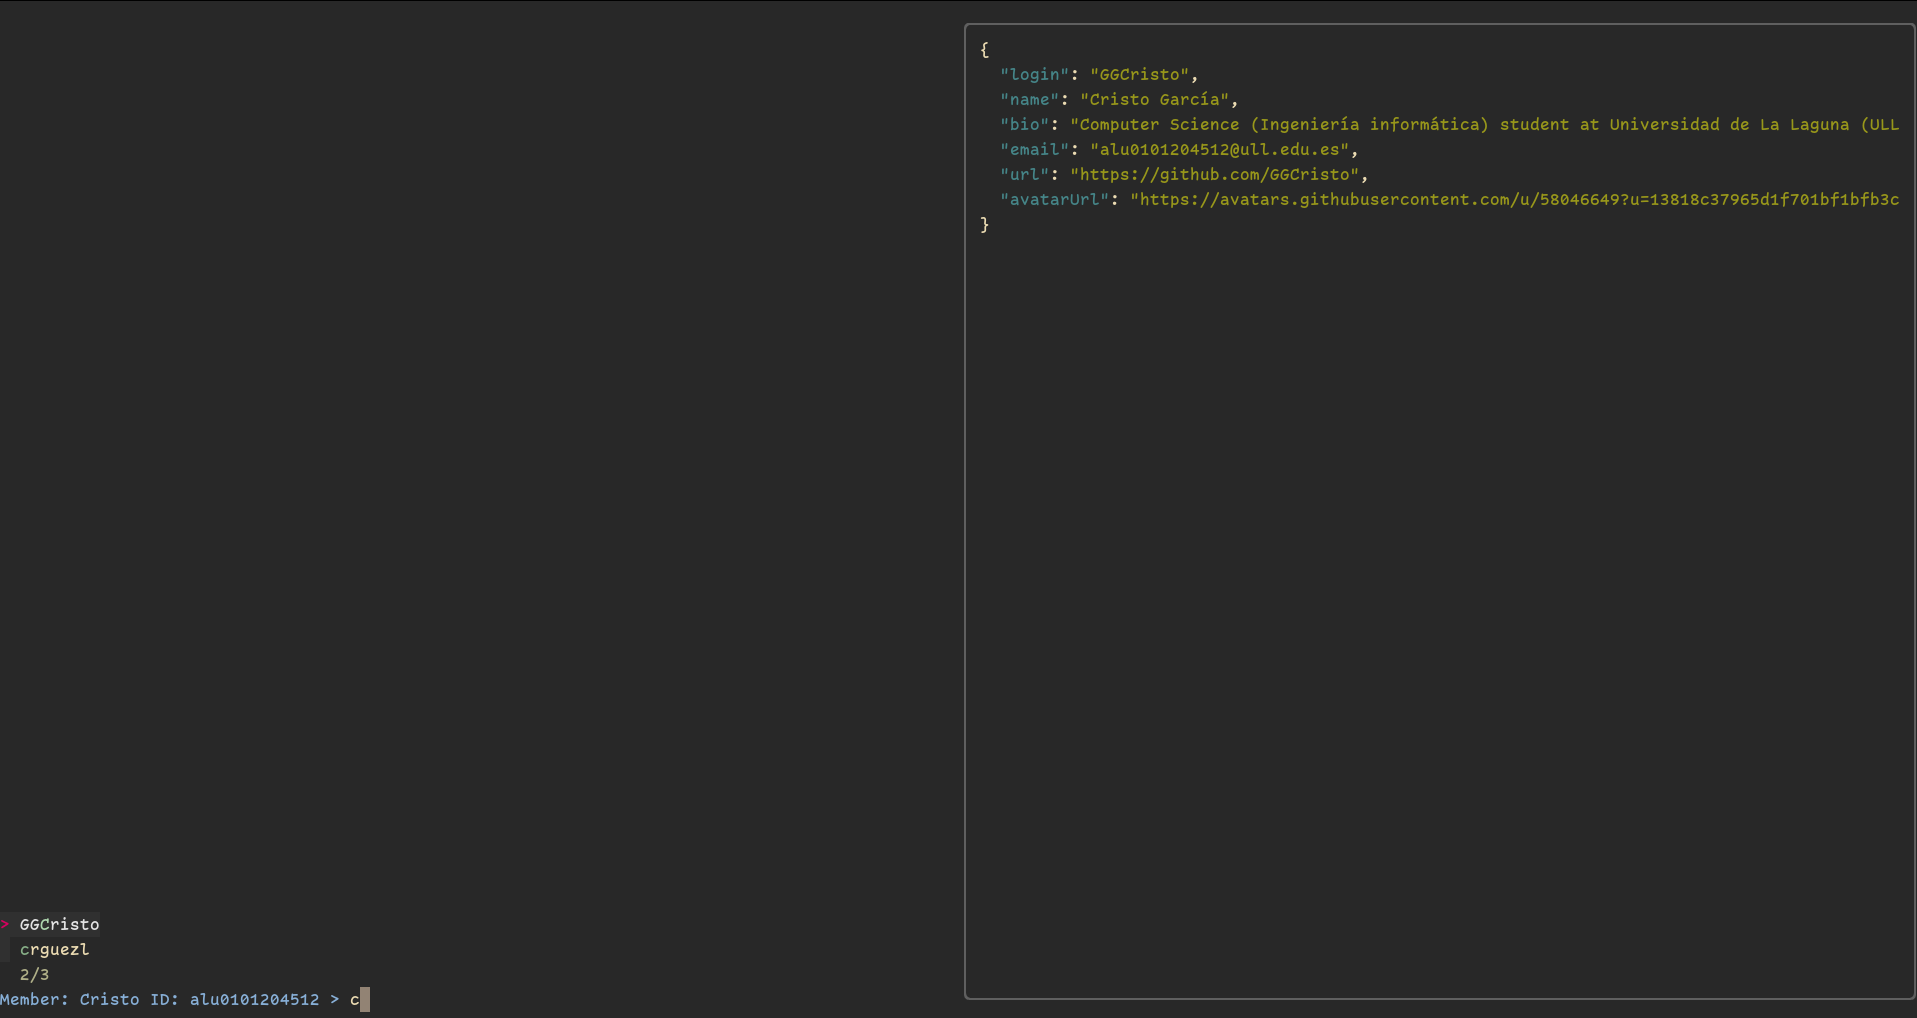
\includegraphics[width=\textwidth]{images/interface-log.png}}
    \caption{gh edu data log. Interfaz principal}
    \label{fig:interface-log}
\end{figure}

\begin{figure}[H]
    \centering
    \makebox[\textwidth][c]{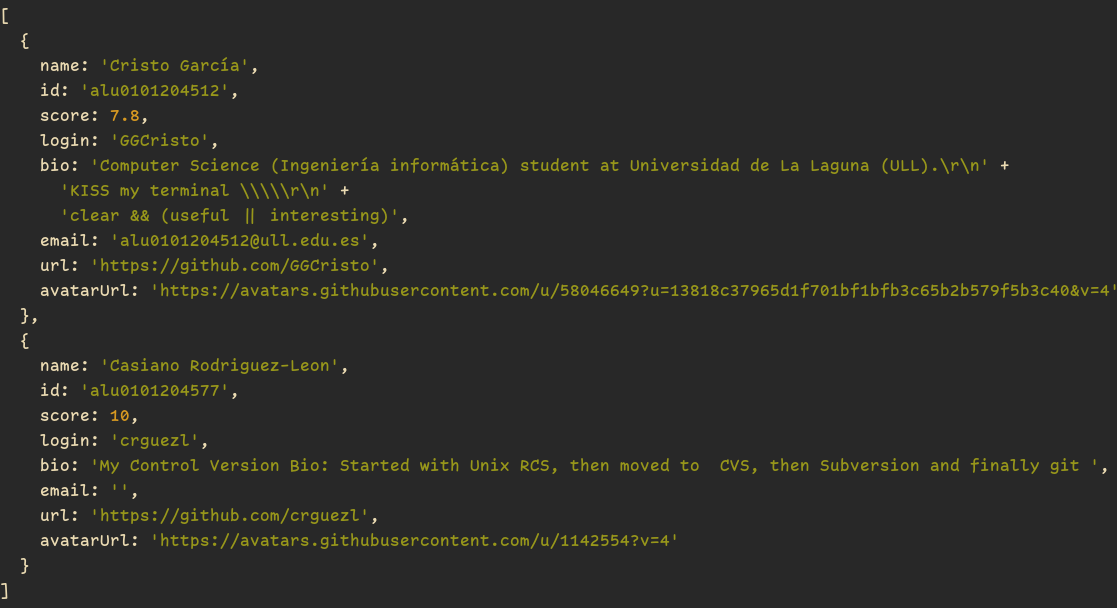
\includegraphics[width=\textwidth]{images/result-log.png}}
    \caption{gh edu data log. Resultado}
    \label{fig:result-log}
\end{figure}

Tiene los siguientes \verb|flags| para modificar su comportamiento:
\begin{figure}[H]
    \centering
    \makebox[\textwidth][c]{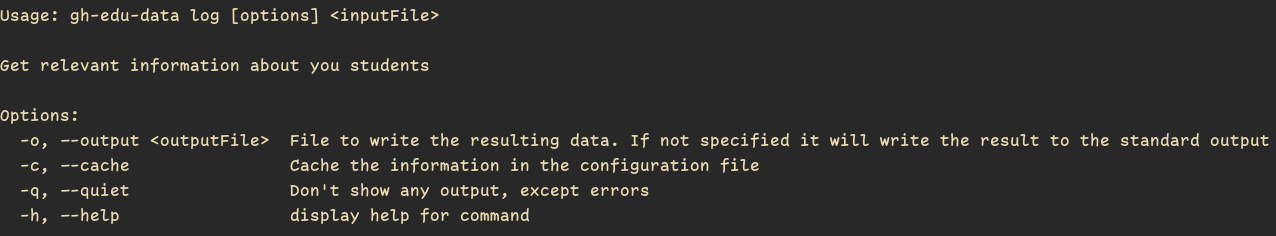
\includegraphics[width=\textwidth]{images/data-log-help.png}}
    \caption{gh edu data log. Ayuda}
    \label{fig:data-log-help}
\end{figure}

Estos \verb|flags| se comportan igual que en el resto de subcomandos, a excepción de \textbf{c, -{}-cache}, en cuyo caso, estamos indicando de que queremos guardar el resultado en una \gls{cache} en el fichero data.json. Un ejemplo del resultado se puede ver en la figura \ref{fig:data}

\subsection{El subcomando {\tt teams}}
Una de las estrategias que suelen utilizar los profesores para tener identificados a los alumnos es que en la primera práctica de la asignatura se procede a crear una asignación de GH Classroom de este modo:
\begin{enumerate}
    \item Usando una asignación de GH Classroom crear una tarea de equipo
    \item Los equipos serán individuales formados por un solo alumno
    \item Cada alumno cuando acepta la asignación crea su equipo le debe dar el nombre según las instrucciones que le haya dado el profesor
\end{enumerate}

Un ejemplo de tal instrucción del profesor sobre el nombre del equipo podría ser: 

"El nombre del equipo debe estar formado por el nombre y apellidos del alumno separado por guiones, seguido del identificador de la universidad. No use tildes ni caracteres especiales".

Por ejemplo para un. alumno dela ULL podría ser algo como \verb|cristo-garcia-gonzalez-alu0101204512|. 

El comando viene gobernado por la expresión regular con paréntesis con nombre 
especificada en la entrada \verb|teamR| del fichero de configuración:
\begin{verbatim}
➜  gh-edu-data git:(casiano) ✗ gh edu get -c | jq '.teamR'
"(?<name>.+)[-_](?<id>.+)"
➜  gh-edu-data git:(casiano) ✗ gh edu get -t
(?<name>.+)[-_](?<id>.+)
\end{verbatim}
Esta expresión regular permite decidir que \verb|name| es la primera parte \verb|cristo-garcia-gonzalez| y que \verb|id| es \verb|alu0101204512|.

\verb|teams| es un comando que tiene el mismo objetivo que \verb|log|, pero se aprovecha de esta estrategia, para que la obtención y búsqueda de dicha información sea inmediata.

El comando actúa sobre la organización por defecto. 
Supongamos fijada la organización de una cierta clase:

\begin{verbatim}
➜  gh-edu-data git:(casiano) ✗ gh edu get -o
ULL-ESIT-PL-2122
\end{verbatim}

El comando tiene las siguientes opciones:

\begin{verbatim}
➜  gh-edu-data git:(casiano) ✗ gh edu data teams -h
Usage: gh-edu-data teams [options]

Get relevant information about you students using teams

Options:
  -o, --output <outputFile>  File to write the resulting data. If not specified
                             it will write the result to the standard output
  -c, --cache                Cache the information in the configuration file
  -q, --quiet                Don't show any output, except errors
  -h, --help                 display help for command
\end{verbatim}

Entonces cuando se ejecuta:

\begin{verbatim}
➜  gh-edu-data git:(casiano) ✗ gh edu data teams
\end{verbatim}

Se conecta a la API de GH para obtener los equipos de un solo miembro he intenta obtener del nombre y propiedades de los equipos de un solo miembro la información necesaria.

Saldrá por stderr mensajes de advertencia para los equipos con mas de un miembro, como este::

\begin{verbatim}
➜  gh-edu-data git:(casiano) ✗ gh edu data teams
Warning! Teams with several members not included in the identification process: {
  "casiano-rodriguez-leon-crguezl": [
    "https://github.com/crguezl",
    "https://github.com/algorithms-ull"
  ]
}
\end{verbatim}

y por stdout saldrá algo como esto:

\begin{verbatim}
[
  {
    "url": "https://github.com/AdalDiazFarina",
    "email": "",
    "nameInGH": "Adal Díaz Fariña",
    "name": "adal-diaz-fariña",
    "id": "alu0101112251"
  },
  ... etc.
  {
    "url": "https://github.com/CorEHarD5",
    "email": "sergiodlbg@gmail.com",
    "nameInGH": "alu0100953275",
    "name": "sergio-barrera-garcia",
    "id": "alu0100953275"
  }
]
\end{verbatim}

\subsection{El subcomando {\tt team-add}}
Este subcomando fue creado como respuesta al subcomando \verb|teams| con la intención de también facilitar el trabajo a los alumnos, a la hora de crear los equipos en la organización.

Se aprovecha del campo \verb|teamR| para saber que datos pedirle al alumno. Por ejemplo, si se tiene en \verb|teamR| el siguiente valor \verb|(?<name>.*?)\.(?<id>.*?)\.(?<age>.*[^s*])|. El programa le preguntará al alumno por \verb|name|, \verb|id| y \verb|age|. Y creará un equipo en la organización especificada por \verb|defaultOrg|, con dichos datos y el alumno como miembro.

\begin{figure}[H]
    \centering
    \makebox[\textwidth][c]{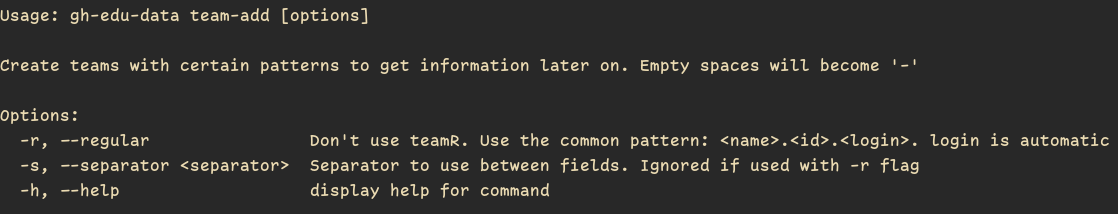
\includegraphics[width=\textwidth]{images/team-add-help.png}}
    \caption{Ayuda para subcomando team-add}
    \label{fig:team-addHelp}
\end{figure}

\begin{itemize}
    \item \textbf{-r, -{}-regular.} Ignora el campo \verb|teamR| y el flag \textbf{-s, -{}-separator}. Le pregunta al alumno por su nombre e identificador y crea un equipo con dicha información, más su identificación en GitHub. El separador es \lq.\rq. Se ha considerado que este patrón es lo suficientemente conveniente, para justificar un \verb|flag| exclusivo para él.
    \item \textbf{-s, -{}-selector.} No se ha encontrado una manera fiable de deducir el selector a partir de \verb|teamR|, por lo que el alumno tendrá que especificarlo con este \verb|flag|. Si se omite, el programa le preguntará al usuario de forma interactiva.
\end{itemize}

\section{La Extensión {\tt plagiarism}}
Es una extensión para detectar el porcentaje de similitud en las tareas de los alumnos. Se puede usar principalmente para ayudar al profesor a detectar plagio.

Genera un grafo mostrando los porcentajes y el número de líneas que son similares entre cada par de alumnos, y un informe con un enlace para ver las similitudes del código fuente.\\
Es necesario tener instalados varías dependencias:
\begin{enumerate}
    \item \textbf{MOSS (Measure Of Software Similarity)\cite{MOSS} script.} El usuario tiene que solicitar un fichero en el que viene incluido la \emph{key}/\emph{id} correspondiente. Los pasos del proceso están en su \href{https://theory.stanford.edu/~aiken/moss/}{página web}.
    \item \textbf{Perl.} Para poder ejecutar el script de \verb|MOSS|.
    \item \textbf{mossum\cite{mossum}.} Para generar el grafo con los datos de \verb|MOSS|.
\end{enumerate}
\verb|fzf| es opcional
\begin{figure}[H]
    \centering
    \makebox[\textwidth][c]{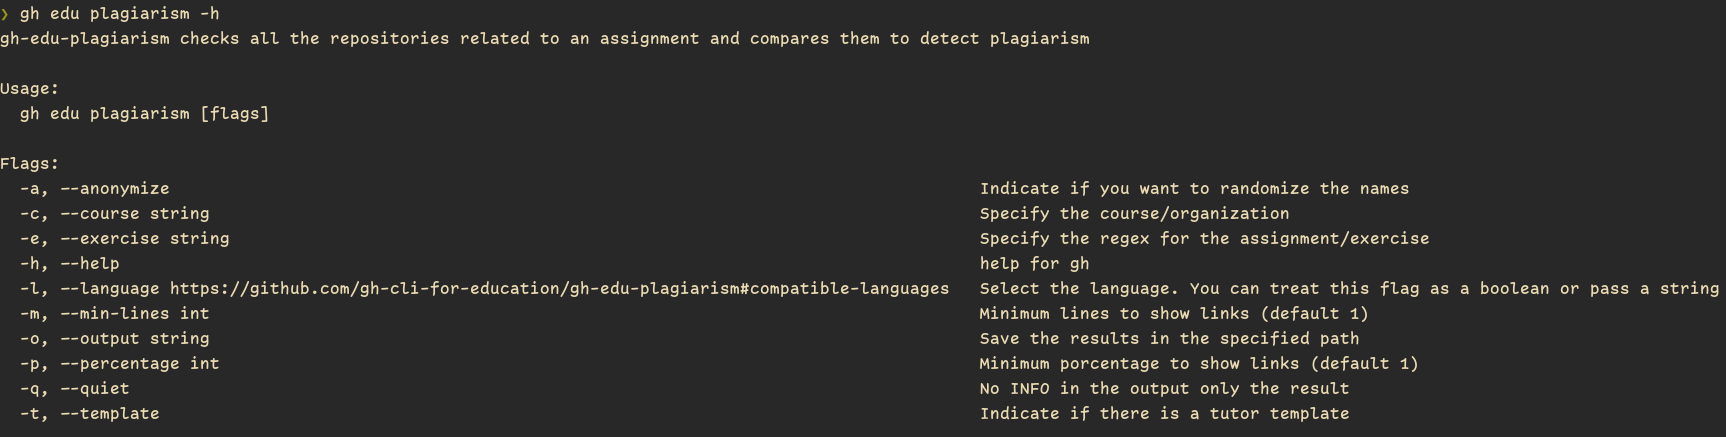
\includegraphics[width=\textwidth]{images/plagiarism-help.png}}
    \caption{Ayuda de gh edu plagiarism}
    \label{fig:plagiarismHelp}
\end{figure}

\begin{itemize}
    \item \textbf{-a, -{}-anonymize}, muestra el grafo con nombres falsos aleatorios. Se podría usar en caso de que el profesor quiera mostrar el grafo a la clase.\\
    \emph{Nota: Este comando solo se aplica al grafo, el informe se queda intacto, ya que está destinado a ser consumido únicamente por el profesor}
    \item \textbf{-c, -{}-course <course>}. La organización se puede indicar con este flag, y toma prioridad con respecto al archivo de configuración.
    \item \textbf{-e, -{}-exercise <exercise>}. La expresión regular para la tarea se puede indicar con este flag, y toma prioridad con respecto al archivo de configuración.
    \item \textbf{-l, -{}-language <language>}. Indica el lenguaje de programación utilizado.\\
    A pesar de que esta sea un campo obligatorio para que funcione el programa, si se omite se pedirá más tarde de forma interactiva con \verb|fzf|
    
    Se aceptan los mismos lenguajes que \verb|MOSS| acepta, los cuales son: c, cc (C++), java, ml (Meta Language), pascal, ada, lisp, scheme, haskell, fortran, ascii, vhdl, perl, matlab, python, mips, prolog, spice, vb (Visual Basic), csharp (C\#), modula2, a8086 (8086 assembly), javascript, plsql (PL/SQL), verilog.
    \item \textbf{-m, --min-lines <lines> (Por defecto: 1)}. Indica cuál es el número mínimo de líneas que deben ser similares para que el estudiante salga en el grafo.
    \item \textbf{-o, --output <path>}. Indica donde se quiere guardar el resultado. El informe y el grafo se guardan en el directorio temporal del sistema hasta la siguiente ejecución, utilizando este flag se puede indicar donde guardar los resultados de forma persistente.
    \item \textbf{-p, -{}-percentage <percentage>(Por defecto: 1)}. Indica cuál es el porcentaje mínimo de similitud entre los pares para mostrar en el grafo.
    \item \textbf{-q, -{}-quiet}. No se muestra ninguna información, aparte del informe final. Útil para redirigir el informe a otro fichero.
\end{itemize}
%%%%%%%%%%%%%%%%%%%%%%%%%%%%%%%%%%%%%%%%%%%%%%%%%%%%%%%%%%%%%%%%%%%%%%%%%%%%%%%
\newpage{\pagestyle{empty}}
\thispagestyle{empty}

\chapter{\LARGE Diseño}
\label{chapter:tres}

El diseño del comando gh owner figura \ref{fig:ghOwner} se ha adaptado cuidadosamente al estilo de diseño de la GitHub CLI, manteniendo la coherencia con la estructura y usabilidad de la herramienta. Mientras que algunos comandos de gh incluyen subcomandos para organizar múltiples funcionalidades, en este caso se optó por implementar un único comando sin subcomandos. Esta decisión se tomó porque todas las funcionalidades requeridas se pueden resolver eficientemente mediante el uso de flags, simplificando así la sintaxis y mejorando la experiencia del usuario al reducir la complejidad operativa.

\begin{figure}[H]
  \begin{lstlisting}[language=Bash]
    The owner command allows you to manage the default owner for GitHub CLI commands.

      USAGE
        gh owner [OWNER] | [flags]

      FLAGS
        -l, --list     List organizations
        -s, --select   Interactively select a default owner
        -u, --unset    Unset the default owner

      INHERITED FLAGS
        --help   Show help for command

      ARGUMENTS
        You can specify an owner as an argument or use the --list, --select, or --unset flags.
        Any of these options can be used, but only one at a time.

      EXAMPLES
        $ gh owner
        $ gh owner [ORGANIZATION | USER]
        $ gh owner --list
        $ gh owner --select
        $ gh owner --unset

      LEARN MORE
        Use `gh <command> <subcommand> --help` for more information about a command.
        Read the manual at https://cli.github.com/manual
  \end{lstlisting}
  \caption{Comando gh owner}
  \label{fig:ghOwner}
\end{figure}

%%%%%%%%%%%%%%%%%%%%%%%%%%%%%%%%%%%%%%%%%%%%%%%%%%%%%%%%%
\newpage{\pagestyle{empty}}
\thispagestyle{empty}

\chapter{\LARGE Implementación}
\label{chapter:cuatro}

En este capítulo se abordará como preparar el entorno para instalar y ejecutar el comando `gh owner` en la GitHub CLI. Además de explicar el desarrollo del comando y las dificultades encontradas.

\section{Entorno}
\subsection{Instalar GO}
El primer paso para utilizar el comando es asegurarse de que Go (Golang) está instalado en el sistema. Para ello, siga estos pasos:

\begin{enumerate}
  \item Descargue la última versión de Go desde la página oficial: https://golang.org/dl/.
  \item Siga las instrucciones de instalación correspondientes a su sistema operativo (Windows, macOS, Linux).
  \item Verifique la instalación abriendo una terminal y ejecutando el siguiente comando:
        \begin{verbatim}
          go version
        \end{verbatim}
\end{enumerate}

Si Go está instalado correctamente, verá una salida con la versión de Go instalada.

\subsection{Descargar el repositorio}

Dado que este proyecto no es una modificación directa de la GitHub CLI oficial, es necesario clonar el repositorio desde un fork y acceder a la rama de desarrollo. Para ello, siga los siguientes pasos:

\begin{enumerate}
  \item Abra una terminal y clone el repositorio desde el fork con el siguiente comando:
        \begin{verbatim}
          git clone git@github.com:gh-cli-for-education/cli.git
        \end{verbatim}
  \item Acceda al directorio del repositorio clonado.
        \begin{verbatim}
          cd cli
        \end{verbatim}
  \item Cambie a la rama de desarrollo específica:
        \begin{verbatim}
          git checkout gh-owner-dev
        \end{verbatim}
\end{enumerate}

\subsection{Compilar el proyecto}

Una vez dentro del repositorio clonado, puede compilar el proyecto utilizando el comando `make`. Siga estos pasos:

\begin{enumerate}
  \item Asegúrese de estar en el directorio raíz del repositorio clonado.
  \item Ejecute el comando `make` para iniciar el proceso de compilación. Este comando se encargará de construir el proyecto y generar los binarios necesarios.
  \item Después de la compilación exitosa, puede utilizar el binario generado para ejecutar el comando. En lugar de utilizar el comando `gh` estándar, utilice el binario ubicado en el directorio `bin` del proyecto:
        \begin{verbatim}
          ./bin/gh <subcomando>
        \end{verbatim}
\end{enumerate}

Con estos pasos, el entorno estará configurado correctamente y podrá empezar a utilizar el comando desarrollado.

\section{Desarrollo del comando}

El comando `gh owner` fue desarrollado siguiendo las pautas y estructura de la GitHub CLI oficial. Para ello, se creó un nuevo subcomando dentro del proyecto existente y se implementó la lógica necesaria para obtener la información del propietario de un repositorio. Todo esto se hizo en dos grandes pasos, primero el comando y su lógica para guardar el OWNER por defecto, y en segundo lugar modificar los comandos ya existentes de `gh` para que utilicen el OWNER guardado.

\subsection{Creación del subcomando `gh owner`}
Para crear un nuevo subcomando en la GitHub CLI, se deben seguir los siguientes pasos:

\begin{enumerate}
  \item Crear un nuevo archivo en el directorio `pkg/cmd/owner` con el nombre `owner.go`. Este archivo contendrá la lógica del subcomando `gh owner`.
  \item Definir la estructura del subcomando, incluyendo la información necesaria para su uso y descripción.
  \item Implementar la lógica del subcomando, que en este caso consiste en obtener el propietario de un repositorio y guardarlo en una variable global.
  \item Registrar el subcomando en el archivo `pkg/cmd/root.go` para que sea reconocido por la GitHub CLI.
  \item Probar el subcomando ejecutando `gh owner` en la terminal y verificando que la información del propietario se muestre correctamente.
\end{enumerate}

Ya teniendo el comando creado lo más importante de la lógica es la query para obtener los OWNERS desde GitHub en la figura \ref{fig:queryOwners}. Cabe destacar que gracias a la estructura de la GitHub CLI se crea un `cachedClient` que permite guardar el resultado de la query por el tiempo que sea especificado, en este caso una semana. Por otra parte importante iterar la query las veces necesarias para obtener todos los OWNERS ya que el límite está en 100 por query.

\begin{figure}[H]
  \begin{lstlisting}[language=GO]
    query := `query OrganizationList($user: String!, $limit: Int!, $endCursor: String) {
      user(login: $user) {
        login
        organizations(first: $limit, after: $endCursor) {
          totalCount
          nodes {
            login
          }
          pageInfo {
            hasNextPage
            endCursor
          }
        }
      }
    }`
  \end{lstlisting}
  \caption{Query para obtener los OWNERS de un usuario}
  \label{fig:queryOwners}
\end{figure}

Respecto a cómo guardar el OWNER figura \ref{fig:saveOwner}, se ha optado por usar la estructura del objeto `Config` que se haya en el `Factory`, siendo así que se acaba guardando en el archivo `~/.config/gh`.

\begin{figure}[H]
  \begin{lstlisting}[language=GO]
    func setDefaultOwner(opts OwnerOptions, ownerList *OrganizationList) error {
      // Get the config object to be able to save the owner
      cfg, err := opts.Config()
      if err != nil {
        return err
      }

      // Check if owner is in the list of organizations
      found := false
      for _, org := range ownerList.Organizations {
        if org.Login == opts.Owner {
          found = true
          break
        }
      }

      if !found {
        fmt.Fprintf(opts.IO.Out, "Owner %s not found\n", opts.Owner)
      } else {
        // Se guarda y escribe en el archivo ~/.config/gh
        cfg.Set("", "gh-owner", opts.Owner)
        err = cfg.Write()
        if err != nil {
          return err
        }
        fmt.Fprintf(opts.IO.Out, "Default owner set to %s\n", opts.Owner)
      }

      return nil
    }
  \end{lstlisting}
  \caption{Función para guardar el OWNER por defecto en la configuración de la gh}
  \label{fig:saveOwner}
\end{figure}



%%%%%%%%%%%%%%%%%%%%%%%%%%%%%%%%%%%%%%%%%%%%%%%%%%%%%%%%%
\newpage{\pagestyle{empty}}
\thispagestyle{empty}

\chapter{\LARGE Conclusiones y líneas futuras}
\label{chapter:Resultados}

``Software Engineering Is Programming Integrated Over Time'' \label{conclusion}

\bigskip
Lo que más resalto en este trabajo de fin de grado ha sido la tarea de diseñar un ecosistema modulable desde cero con unas metas marcadas y con el ideal de crear un software que no necesite de cambios en su estructura para crecer, que sea simple e intuitivo, pero útil y que permita la colaboración. Conseguir todas estas características ha requerido una amplia etapa de diseño y prototipado donde las ideas se implementaban y descartaban por igual.\\
También otro apartado que consumió bastante tiempo fue el manejo de errores. Al ser una aplicación que realiza muchas llamadas, lee y escribe de ficheros y le pide \emph{input} al usuario, hay muchos puntos donde la aplicación puede fallar. Manejar estos errores y pulir la aplicación en general es trabajo que no genera un resultado inmediato, pero hace que la aplicación sea más mantenible y estable.\\
Por otro lado, me siento muy afortunado de haber podido trabajar con tecnologías con las que me siento cómodo como JavaScript, Go y \verb|fzf|, pero han sido más las que he aprendido y dada la buena experiencia que he tenido con: \verb|jq|, \verb|gh cli| y \verb|GraphQL| comentar que seguramente las utilice en futuros proyectos.\\
No obstante, me apena no haber podido cumplir con el objetivo de interoperabilidad entre comandos. El comando \verb|view| se podría beneficiar enormemente si pudiese leer de la \emph{standard input} para recibir información de un comando como \verb|data|, pero preferí enfocar el tiempo en mejorar la calidad y usabilidad de todo el ecosistema.\\
El trabajo de fin de grado está terminado, pero el proyecto puede crecer tanto como desee. Este tipo de proyecto requiere de trabajo constante y prolongado para que tenga acogida en la comunidad. Mis intenciones son seguir contribuyendo a este proyecto y tomarlo como mi proyecto personal y mi vía de contribución al open source.

%%%%%%%%%%%%%%%%%%%%%%%%%%%%%%%%%%%%%%%%%%%%%%%%%%%%%%%%%
\newpage{\pagestyle{empty}}
\thispagestyle{empty}

\chapter{\LARGE Summary and Conclusions}
\label{chapter:Conclusiones}

``Software Engineering Is Programming Integrated Over Time''

\bigskip


%%%%%%%%%%%%%%%%%%%%%%%%%%%%%%%%%%%%%%%%%%%%%%%%%%%%%%%%%
\newpage{\pagestyle{empty}}
\thispagestyle{empty}

\chapter{\LARGE Presupuesto}
\label{chapter:presupuesto}

Todas las tecnologías usadas son \emph{open source} y gratuitas y se presupone que el ordenador usado es personal, por lo que no se incluye en el presupuesto\\
El hipotético saldo son 15 euros la hora

\begin{comment}
\begin{center}
\begin{tabu} to 0.8\textwidth {| X[l] | X[l] | X[l] |}
 \hline
 \multicolumn{1}{|c|}{\bf Coste} & \multicolumn{1}{|c|}{\bf Tipos} & \multicolumn{1}{|c|}{\bf Descripción} \\
 \hline 4500 & Formación y Diseño & La formación en nuevas tecnologías y el diseño de la aplicación han consumido un tiempo sustancial de 300 horas\\
 \hline
 3000  & Desarrollo de los prototipos y aplicación final & Aproximadamente se ha dedicado unas 200 horas\\
 \hline
 120 & Elaboración del informe y conclusiones  & Al tratarse de un ecosistema \emph{open source} lanzado a un público general, la documentación es importante, por lo que se ha desarrollado no solo este informe. si no documentación para usuario y desarrolladores en los respectivos repositorios. \\
 \hline
\end{tabu}
\end{center}
\end{comment}
\begin{table}[H]
    \centering
    \begin{tabular}{|m{1cm}|m{4cm}|m{10cm}|}
    \hline
    \textbf{Coste} & \textbf{Tipos} & \textbf{Descripción}\\
    \hline
    4500 & Diseño y planificación & Incluyendo el tiempo invertido en investigación de las nuevas tecnologías necesarias y el diseño y planificación de la aplicación se ha consumido un tiempo sustancial de 300 horas\\
    \hline
    3000  & Desarrollo de los prototipos y aplicación final & Aproximadamente se ha dedicado unas 200 horas\\
    \hline
    495 & Elaboración del informe y conclusiones  & Al tratarse de un ecosistema \emph{open source} lanzado a un público general, la documentación es importante, por lo que se ha desarrollado no solo este informe. si no documentación para usuario y desarrolladores en los respectivos repositorios. Necesitando un total de 33 horas\\
    \hline
    \end{tabular}
    \caption{Tabla del presupuesto}
    \label{tab:budget}
\end{table}

\begin{comment}
   \begin{table}[htb]
   \centering
   \caption{Presupuesto}
   \label{table:presupuesto}
\end{table} 
\end{comment}

Esto supone un presupuesto total de, 7995 euros en un periodo de 3 meses

%%%%%%%%%%%%%%%%%%%%%%%%%%%%%%%%%%%%%%%%%%%%%%%%%%%%%%%%%
\newpage{\pagestyle{empty}\cleardoublepage}
\thispagestyle{empty}

\begin{appendix}

\chapter{\LARGE Repositorios del ecosistema}
\label{appendix:1}
Se adjuntan los enlaces a los repositorios de GitHub de los diferentes códigos en los que se ha trabajado.

\begin{itemize}
  \item XXXX
  El código de \verb|gh-edu| se encuentra en

  \href{https://github.com/gh-cli-for-education/gh-edu}{{\tt https://github.com/gh-cli-for-education/gh-edu}}

  
\end{itemize}

\end{appendix}
%\printnoidxglossaries
\printglossary[title=Glosario, toctitle=Glosario]

%%%%%%%%%%%%%%%%%%%%%%%%%%%%%%%%%%%%%%%%%%%%%%%%%%%%%%%%%%
%\begin{thebibliography}{X}
% Aquí figurará la bibliografía
%\end{thebibliography}
%\bibliographystyle{plain}
\bibliographystyle{unsrt}

\bibliography{memtfg} 
%\bibliography{bib.tex}
%%%%%%%%%%%%%%%%%%%%%%%%%%%%%%%%%%%%%%%%%%%%%%%%%%%%%%%%%%

\end{document}

